\documentclass{beamer}

\usepackage[utf8]{inputenc}
\usepackage{listings}
\usepackage{tikz}
\usepackage{graphicx}

\lstset{basicstyle=\tiny, numberstyle=\tiny,tabsize=1}

\usetheme[navigation]{UMONS}

\title{Est-il possible de duper Google ?}
\subtitle{(JMS 2012)}
\author[X.~Deschuyteneer et H.~Mélot]{X. Deschuyteneer et H. Mélot}
\institute[]{%
  Institut d'informatique\\
  Université de Mons
  \\[2ex]
  \includegraphics[height=4ex]{UMONS+txt}\hspace{2em}%
  \raisebox{-1ex}{\includegraphics[height=6ex]{UMONS_FS}}
}

\date{13 Mars 2012}

\begin{document}

\begin{frame}
  \titlepage
\end{frame}


\begin{frame}
  \tableofcontents[subsectionstyle=hide]
\end{frame}


\section{Introduction}
\subsection{Rôle de Google}

\begin{frame}
  \tableofcontents[currentsection,subsectionstyle=hide]
\end{frame}

\begin{frame}
  \frametitle{Rôle de Google}
  
  
\includegraphics[scale=0.5]{google}\ \\
  \begin{block}{}
    Google est une société qui possède notamment un moteur de recherche.\\
    Son but est de classer des pages web.
  \end{block}
\end{frame}

\begin{frame}
  \frametitle{Rechercher une page dans Google}
  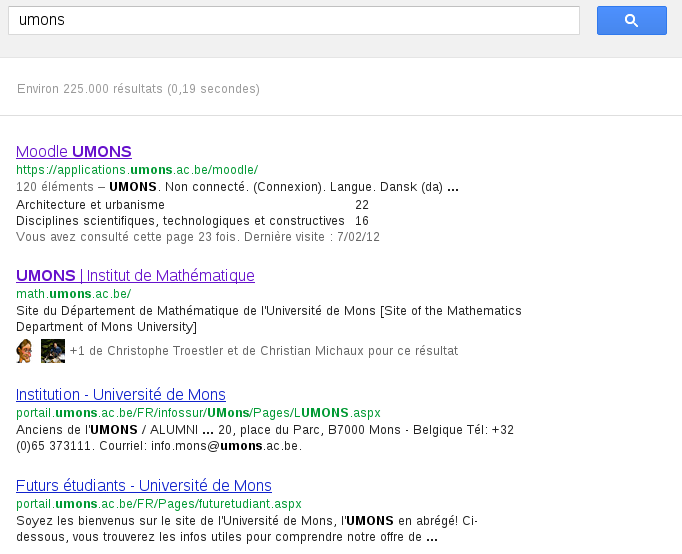
\includegraphics[scale=0.3]{umons_web}
\end{frame}


\begin{frame}
  \frametitle{Exemple de page web}
  \begin{tabular}{cc}
    \begin{minipage}{0.37\linewidth}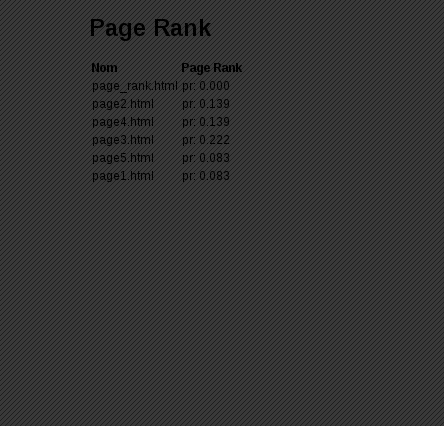
\includegraphics[scale=0.3]{exemple_web}\end{minipage} & \begin{minipage}{0.4\linewidth}\lstinputlisting[language=HTML]{../html/rank.xsl}\end{minipage}
    
\end{tabular}

\end{frame}

\begin{frame}
  \frametitle{Comment Google trouve toute ces pages?}

  
  \begin{block}{Avant}
    Le web était très petit, recenser et classer les pages pouvait
    donc être fait à la page.
  \end{block}
  
  \pause

  \begin{block}{Aujourd'hui}
    Des petits programmes s'occupent de surfer sur internet, de suivre
    les liens, de collecter des données utiles au classement des
    pages.
  \end{block}


\end{frame}


\begin{frame}
  \frametitle{Contexte: Comment classer les pages?}
  
  Pour classer les pages internet, il faut prendre en compte plusieurs
  choses:\\
  
  \begin{itemize}
    \item popularité (trafic)
      \pause
    \item sites de références (gouvernement, Le Monde, etc.)
      \pause
    \item le contenu
      \pause
    \item et la suite?
  \end{itemize}

\end{frame}

\section{Algorithme simple}
\subsection{Idées}


\begin{frame}
  \tableofcontents[currentsection,subsectionstyle=hide]
\end{frame}


\begin{frame}
  \frametitle{Première approche (1/2)}
  
  Voici la représentation de quelques pages internet:\\\ \\
  \pause
  \begin{columns}
    \begin{column}[l]{0.05\linewidth}
      \phantom{``e''}
    \end{column}
    \begin{column}[c]{0.45\linewidth}
      \begin{minipage}{0.45\linewidth}
        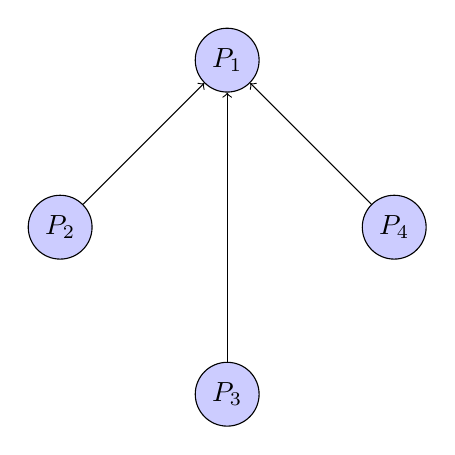
\begin{tikzpicture}[scale=0.5,node distance=3cm, main node/.style={circle,fill=blue!20,draw}]
          
          \node[main node] (1) {$P_1$};
          \node[main node] (2) [below left of=1] {$P_2$};
          \node[main node] (3) [below right of=2] {$P_3$};
          \node[main node] (4) [below right of=1] {$P_4$};
          
          \draw[->] (2) -- (1);
          \draw[->] (3) -- (1);
          \draw[->] (4) -- (1);
          
        \end{tikzpicture}
        
      \end{minipage}
    \end{column}
    \begin{column}[r]{0.65\linewidth}
      \begin{minipage}[t]{0.65\linewidth}
        \pause
        \begin{block}{Question}
          Comment classer ces pages par rapport à leur popularité?
        \end{block}
        \end{minipage}
    \end{column}
  \end{columns}
 
 
\end{frame}

\subsection{Exemple}

\begin{frame}
  \frametitle{Première approche (2/2)}
  \begin{columns}
    \begin{column}[l]{0.1\linewidth}
      \phantom{``pouet''}
    \end{column}
    \begin{column}[c]{0.5\linewidth}
      \begin{minipage}{0.5\linewidth}
        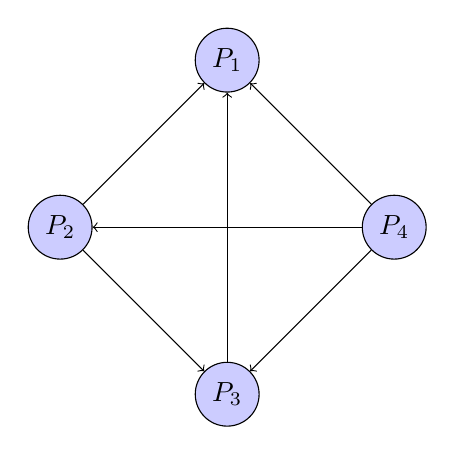
\begin{tikzpicture}[node distance=3cm, main node/.style={circle,fill=blue!20,draw}]
          
          \node[main node] (1) {$P_1$};
          \node[main node] (2) [below left of=1] {$P_2$};
          \node[main node] (3) [below right of=2] {$P_3$};
          \node[main node] (4) [below right of=1] {$P_4$};
          
          \draw[->] (2) -- (1);
          \draw[->] (2) -- (3);
          
          \draw[->] (3) -- (1);
          
          \draw[->] (4) -- (1);    
          \draw[->] (4) -- (2);
          \draw[->] (4) -- (3);
        \end{tikzpicture}
      \end{minipage}
    \end{column}
    \begin{column}[r]{0.65\linewidth}
      \begin{minipage}[t]{0.65\linewidth}
        \pause
        \begin{block}{Question}
          Et ces pages-ci, comment les classer?
        \end{block}
        \end{minipage}
    \end{column}
  \end{columns}
\end{frame}

\begin{frame}
  \frametitle{Duper Google}
  \begin{columns}
    \begin{column}[l]{0.05\linewidth}
      \phantom{``e''}
    \end{column}
    \begin{column}[c]{0.45\linewidth}
      \begin{minipage}{0.45\linewidth}

        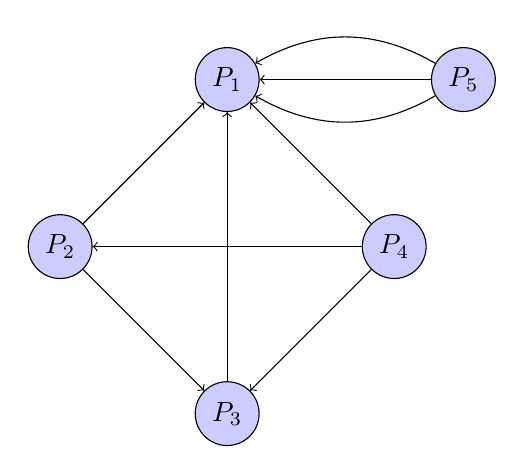
\begin{tikzpicture}[node distance=3cm, main node/.style={circle,fill=blue!20,draw}]
          
          \node[main node] (1) {$P_1$};
          \node[main node] (2) [below left of=1] {$P_2$};
          \node[main node] (3) [below right of=2] {$P_3$};
          \node[main node] (4) [below right of=1] {$P_4$};
          \node[main node] (5) [right of=1] {$P_5$};
          
          \draw[->] (2) -- (1);
          \draw[->] (2) -- (3);
          
          \draw[->] (3) -- (1);
          
          \draw[->] (4) -- (1);    
          \draw[->] (4) -- (2);
          \draw[->] (4) -- (3);
          
          \draw[->] (5) to [out=210,in=330] (1);
          \draw[->] (5) to [out=180,in=0] (1);
          \draw[->] (5) to [out=150,in=30] (1);
        \end{tikzpicture}
      \end{minipage}
    \end{column}
    \begin{column}[r]{0.65\linewidth}
      \begin{minipage}[t]{0.65\linewidth}
        \pause
        \begin{block}{Question}
          Quel serait le classement maintenant?
        \end{block}
        \end{minipage}
    \end{column}
  \end{columns}
\end{frame}

\section{Algorithme final}
\subsection{Notation}

\begin{frame}
  \tableofcontents[currentsection,subsectionstyle=hide]
\end{frame}

\begin{frame}
  \frametitle{Notation}

  \begin{block}{Page rank}
    La \emph{note} d'une page est appelée Page Rank et sera notée $PR(x)$
    pour désigner la note de la page $x$.
  \end{block}

  \pause

  \begin{block}{Liens}
    On notera également $L(x)$ le nombre de liens sortant d'une page
    $x$. 
  \end{block}

  \pause

  \begin{block}{Contrainte}
    On veut imposer $0$ $<$ $PR(x)$ $<$ $1$.\\
    On prend donc comme $PR(x)$ par défaut $\frac{1}{nbr\ pages}$ 
  \end{block}
\end{frame}

\subsection{Exemple}

\begin{frame}
  \frametitle{Notation: Exemple}

    \begin{columns}
    \begin{column}[l]{0.05\linewidth}
      \phantom{``e''}
    \end{column}
    \begin{column}[c]{0.45\linewidth}
      \begin{minipage}{0.45\linewidth}
        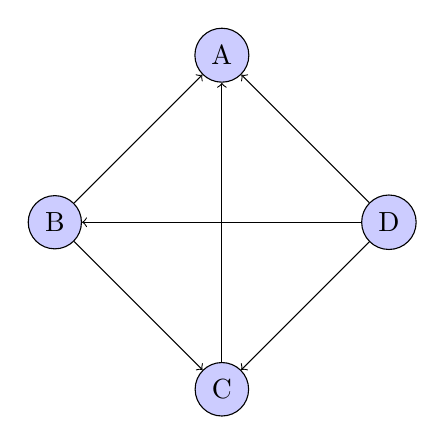
\begin{tikzpicture}[node distance=3cm, main node/.style={circle,fill=blue!20,draw}]
          
          \node[main node] (1) {A};
          \node[main node] (2) [below left of=1] {B};
          \node[main node] (3) [below right of=2] {C};
          \node[main node] (4) [below right of=1] {D};
          
          \draw[->] (2) -- (1);
          \draw[->] (2) -- (3);
          
          \draw[->] (3) -- (1);
          
          \draw[->] (4) -- (1);    
          \draw[->] (4) -- (2);
          \draw[->] (4) -- (3);
        \end{tikzpicture}
      \end{minipage}
    \end{column}
    \begin{column}[r]{0.7\linewidth}
      \begin{minipage}[t]{0.7\linewidth}
        \pause
        \begin{block}{Question}
          Comment calculer $PR(A)$?
        \end{block}
        \pause
        \begin{block}{Réponse}
          $PR(A)$ =\\
          $\frac{PR(B)}{L(B)} + \frac{PR(C)}{L(C)} + \frac{PR(D)}{L(D)}$\\
          = $\frac{0.25}{2} + \frac{0.25}{1} + \frac{0.25}{3}$ = $0.125$
        \end{block}
        \end{minipage}
    \end{column}
  \end{columns}
\end{frame}

\section{Surfer aléatoire}

\begin{frame}
  \tableofcontents[currentsection,subsectionstyle=hide]
\end{frame}

\begin{frame}
  \frametitle{Résumé}

  Pour l'instant nous n'avons pris en compte que des faits:\\
  
  \begin{itemize}
    \item nombre de page
      \pause
    \item nombre de lien entrant
      \pause
    \item nombre de lien sortant
  \end{itemize}

\end{frame}

\begin{frame}
  \frametitle{Principe}

  \begin{block}{Damping factor}
    On va prendre en compte 2 faits courant sur le web, la probabilité
    de cliquer sur un lien pour arriver sur une autre page, noté $d$ et
    la probabilité d'arriver sur une page sans avoir suivit de lien (ie
    $\frac{1 - d}{N}$ avec $N$ le nombre de pages). Des études ont
    montrés qu'une bonne approximation de $d$ était $85\%$.
  \end{block}
\end{frame}

\section{Algorithme réel}
\subsection{Modélisation}

\begin{frame}
  \tableofcontents[currentsection,subsectionstyle=hide]
\end{frame}

\begin{frame}
  \frametitle{Modélisation (1/3)}

   \begin{columns}
    \begin{column}[l]{0.05\linewidth}
      \phantom{``e''}
    \end{column}
    \begin{column}[c]{0.6\linewidth}
      \begin{minipage}{0.6\linewidth}
        Considérons ces pages\\\ \\
        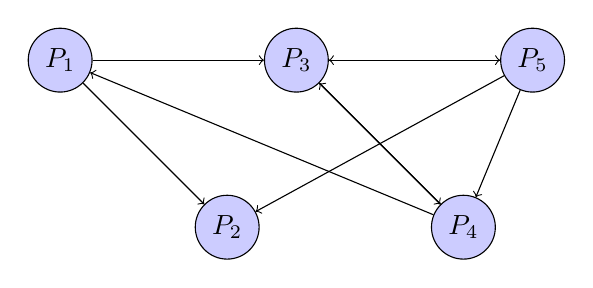
\begin{tikzpicture}[node distance=3cm, main node/.style={circle,fill=blue!20,draw}]
          
          \node[main node] (1) {$P_1$};
          \node[main node] (2) [below right of=1] {$P_2$};
          \node[main node] (3) [right of=1] {$P_3$};
          \node[main node] (4) [below right of=3] {$P_4$};
          \node[main node] (5) [right of=3] {$P_5$};

          \draw[->] (1) -- (2);
          \draw[->] (1) -- (3);
          
          \draw[->] (3) -- (4);
          \draw[->] (3) -- (5);
          
          \draw[->] (4) -- (1);
          \draw[->] (4) -- (3);

          \draw[->] (5) -- (2);
          \draw[->] (5) -- (3);
          \draw[->] (5) -- (4);
          
        \end{tikzpicture}\\
      \end{minipage}
    \end{column}
    \begin{column}[r]{0.6\linewidth}
      \begin{minipage}[t]{0.6\linewidth}
        \pause
        Sous forme de système:\\
        \[ \left \{
          \begin{array}{ c @{ = } l }
            p_1 & \frac{p_4}{2}\\
            p_2 & \frac{p_1}{2} + \frac{p_5}{3}\\
            p_3 & \frac{p_2}{2} + \frac{p_4}{2} + \frac{p_5}{3}\\
            p_4 & \frac{p_3}{2} + \frac{p_5}{3}\\
            p_5 & \frac{p_3}{2}\\
          \end{array}
        \right. \]
        \end{minipage}
    \end{column}
  \end{columns}

  
\end{frame}


\begin{frame}
  \frametitle{Modélisation (3/3)}
  
  Ce système peut être vu sous forme de matrice:\\
  \begin{columns}

    \begin{column}[l]{0.3\linewidth}
      \begin{minipage}{0.3\linewidth}
        \[ \left(
          \begin{array}{ c c c c c}
            0           & 0 & 0           & \frac{1}{2} & 0           \\
            \frac{1}{2} & 0 & 0           & 0           & \frac{1}{3} \\
            \frac{1}{2} & 0 & 0           & \frac{1}{2} & \frac{1}{3} \\
            0           & 0 & \frac{1}{2} & 0           & 0           \\
            0           & 0 & \frac{1}{2} & 0           & \frac{1}{3}
          \end{array} \right)
        \]
      \end{minipage}
    \end{column}

    \begin{column}[r]{0.0001\linewidth}
      \begin{minipage}{0.0001\linewidth}
        .
      \end{minipage}
    \end{column}

    
    \begin{column}[c]{0.05\linewidth}
      \begin{minipage}{0.05\linewidth}
        \[ \left(
          \begin{array}{ c }
            s_1 \\
            s_2 \\
            s_3 \\
            s_4 \\
            s_5
          \end{array} \right)
        \]
      \end{minipage}
    \end{column}

    \begin{column}[r]{0.01\linewidth}
      \begin{minipage}{0.01\linewidth}
          =
      \end{minipage}
    \end{column}

    \begin{column}[r]{0.3\linewidth}
      \begin{minipage}{0.3\linewidth}
        \[ \left(
          \begin{array}{ c }
            s_1 \\
            s_2 \\
            s_3 \\
            s_4 \\
            s_5
          \end{array} \right)
        \]
      \end{minipage}
    \end{column}

  \end{columns}
  
\end{frame}


\begin{frame}
  \frametitle{Résumé}
  
  Ce que nous avons vu:
  
  \begin{enumerate}
    \item page rank basé sur le nombre de lien pointant vers une page
      \pause
    \item pondéré par le nombre de lien sortant
      \pause
    \item vision récursive
      \pause
    \item introduction du damping factor
      \pause
    \item vision matricielle
  \end{enumerate}

\end{frame}

\subsection{Brin et Page}

\begin{frame}
  \frametitle{Algorithme}
  \frametitle{Formule}
  \begin{block}{Brin et Page (1998)}
    \[PR(i) = \frac{1 - d}{N} + d \sum_{j=1}^i {\frac{PR(j)}{l_j}}\]
  \end{block}

  Cette formule du PR donne certaines propriétés à la matrice vue
  précédemment. Le système possède des propriétés très interressantes:\\\ \\
  \begin{itemize}
    \item possède une solution unique
    \item la somme des PR vaut 1
    \item résoudre le système peut être ramené à calculer $M^n$
    \item convergeance très rapide (+/- 100 itérations pour tout le web)
  \end{itemize}

\end{frame}


\end{document}
